\documentclass[aspectratio=169]{beamer}
\usepackage{hyperref}
\usepackage[T1]{fontenc}
\usepackage{NTU}

% Disable auto-generated TOC interstitials to stay within slide budget
\makeatletter
\AtBeginSection[]{}
\AtBeginSubsection[]{}
\makeatother

% Packages
\usepackage{latexsym,amsmath,xcolor,multicol,booktabs}
\usepackage{graphicx,listings}
\usepackage{tikz}
\usetikzlibrary{shapes.geometric,arrows.meta,positioning,calc}

\usepackage[backend=biber,style=numeric]{biblatex}
\addbibresource{references.bib}

\author{Benjamin Oliver Yick (U2120984H)}
\title[Multi-Stakeholder Ethical Decision Framework (MEDF)]{%
  \resizebox{0.95\textwidth}{!}{Multi-Stakeholder Ethical Decision-Making Frameworks (MEDF) for AI Systems}}
\subtitle{Final-Year Project CCDS25-0582}
\institute{College of Computing and Data Science, Nanyang Technological University (Singapore)}
\date{Academic Year 2025/2026}


\begin{document}

\begin{frame}
    \titlepage
    \vspace{-10pt}
    \begin{columns}[c]
        \begin{column}{0.5\textwidth}
            \centering
            {\small Supervisor: Dr.\ Zhang Jiehuang}\\
            {\small Examiner: A/P A S Madhukumar}
        \end{column}
        \begin{column}{0.5\textwidth}
            \centering
            
\includegraphics[width=0.45\linewidth]{images/ntu-logo.png}
        \end{column}
    \end{columns}
\end{frame}
% NOTES: Welcome the examiner and supervisor. State your name and Final-Year Project title.
% Approximately 30 seconds. Transition: "Let me begin by showing you the working platform."


\section{Platform Demo and Problem Context}

% ============================================================
% S2: LIVE PLATFORM DEMO - CONFIGURATION
% ============================================================
\begin{frame}{Live Platform Demo: Evaluation Configuration}
    \begin{columns}[T]
        \begin{column}{0.48\textwidth}
            \begin{itemize}
                \item MEDF evaluates AI systems against multiple governance frameworks simultaneously.
                \item Configurable stakeholder weights model different value systems.
                \item Live at: {\footnotesize\url{https://ccds25-0582-medf-api.streamlit.app/}}.
            \end{itemize}
        \end{column}
        \begin{column}{0.48\textwidth}
            \centering
            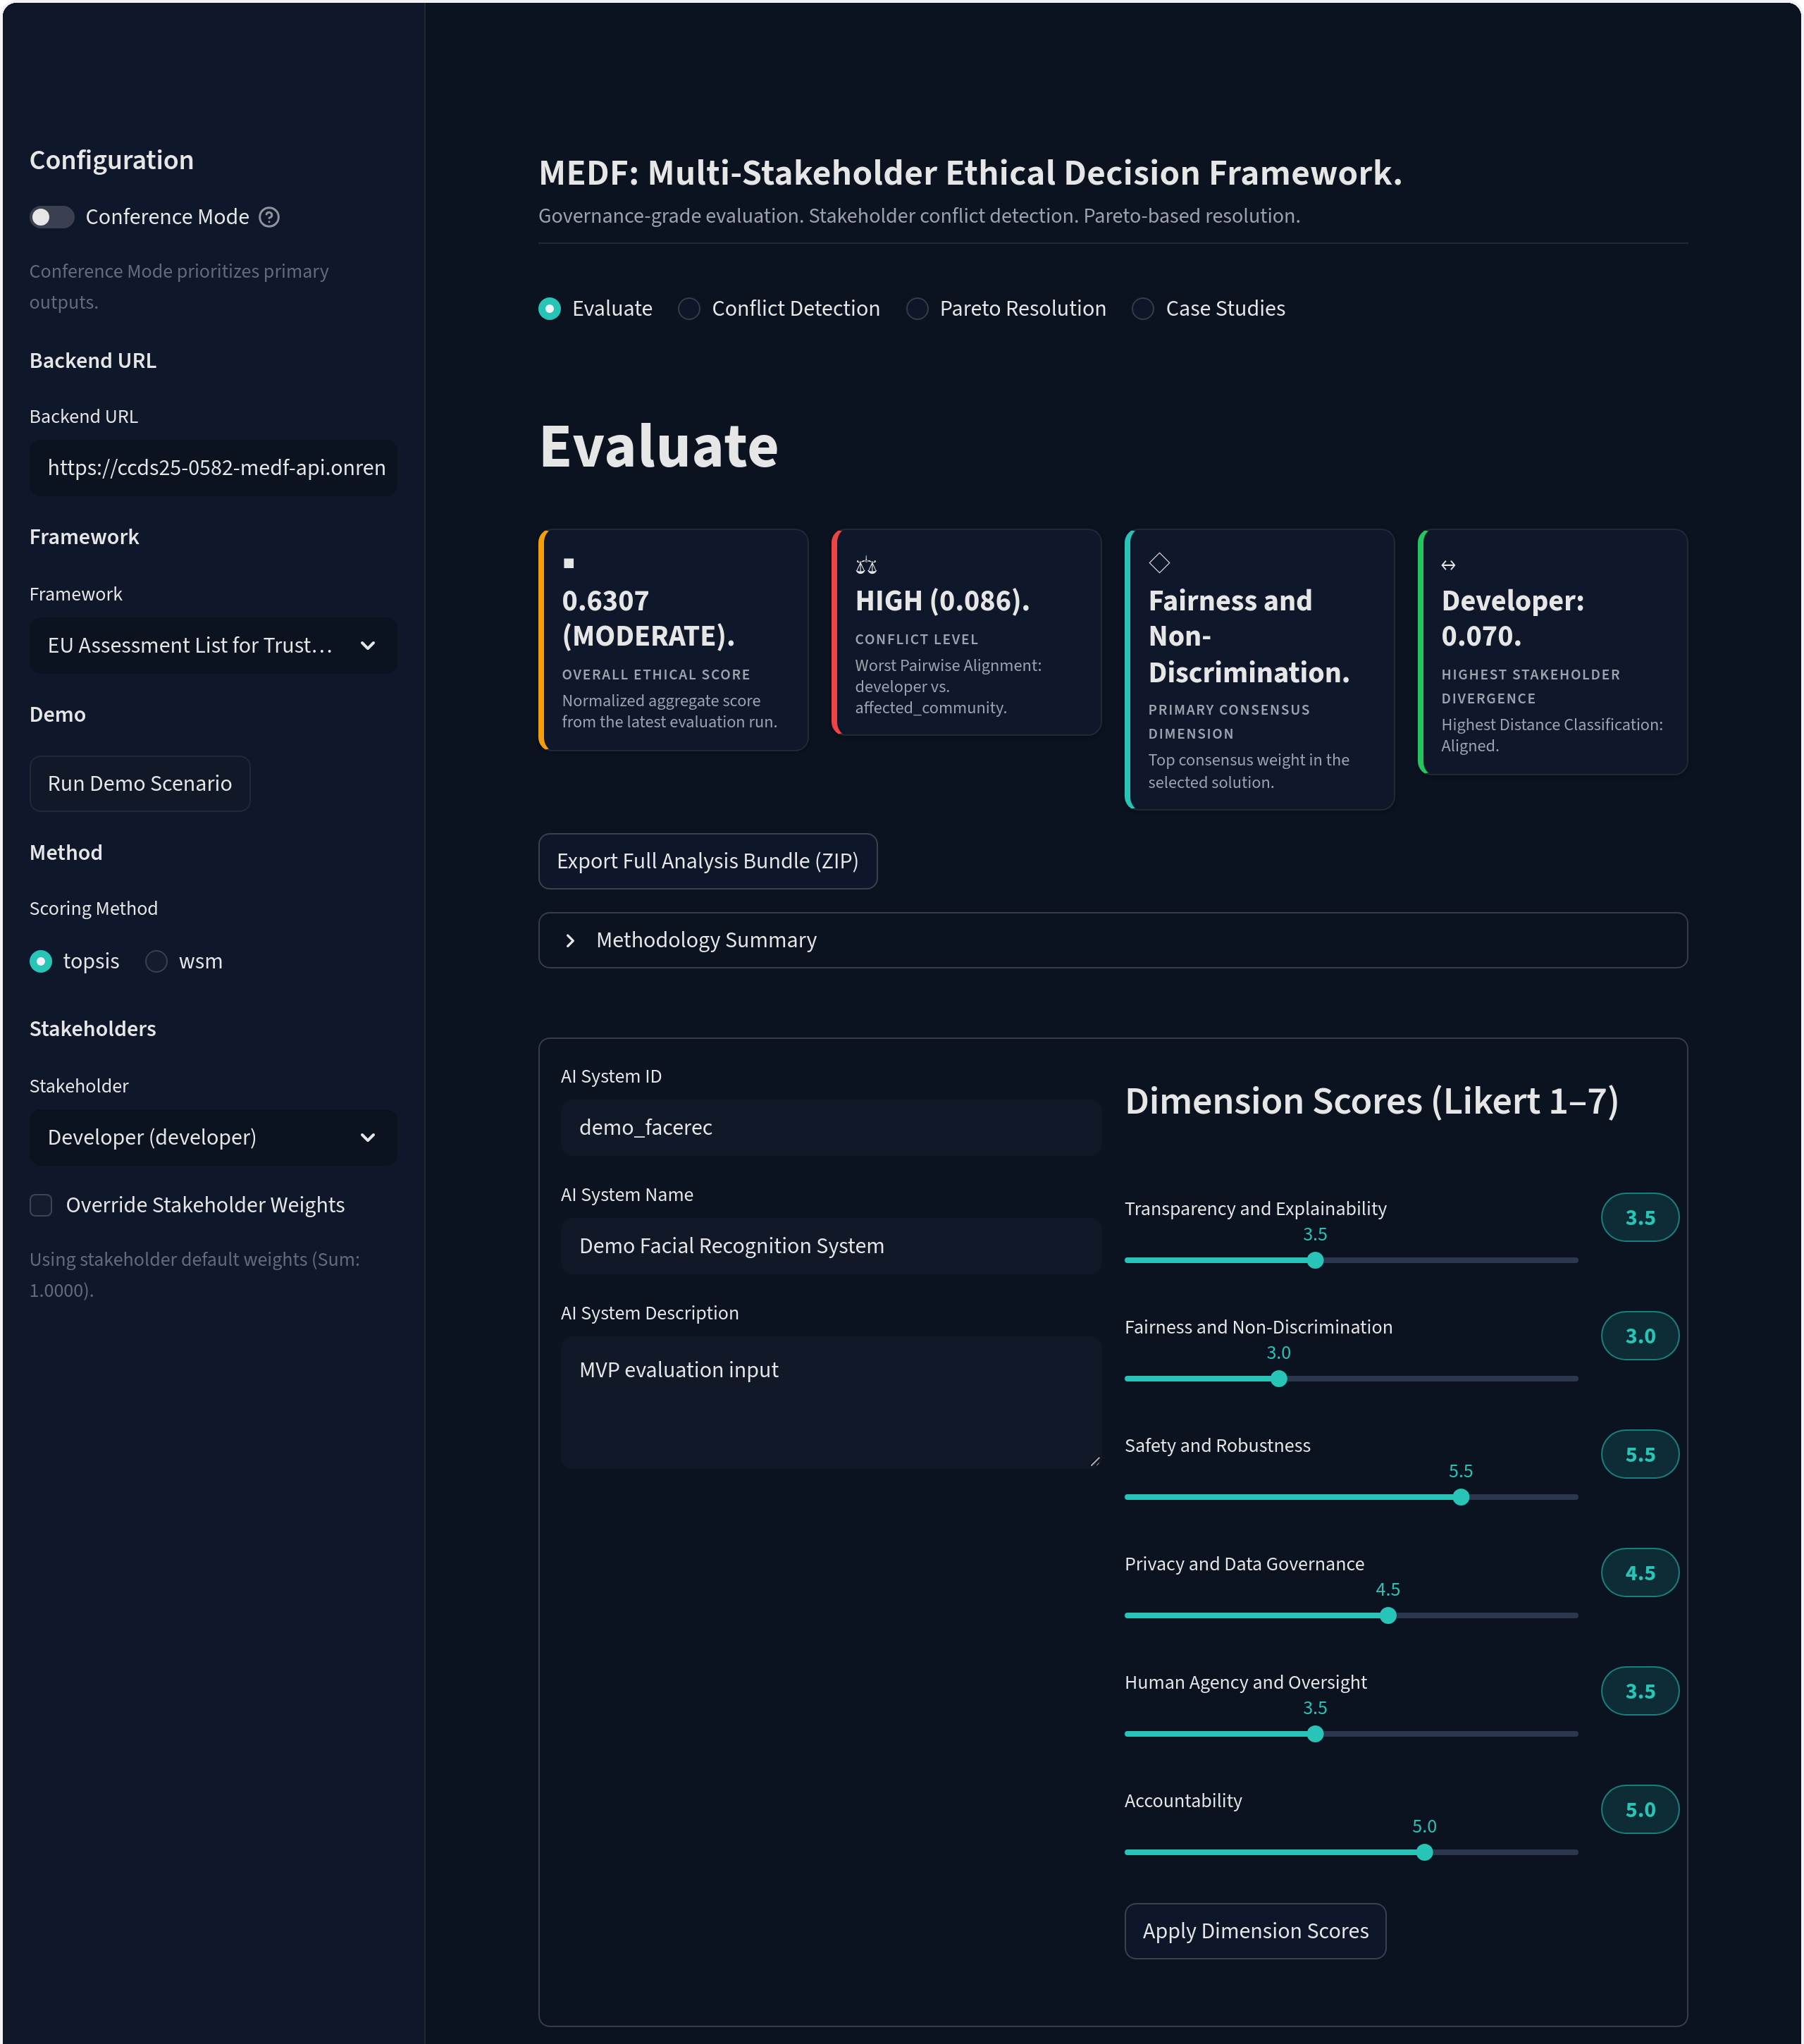
\includegraphics[width=\linewidth,height=0.55\textheight,keepaspectratio]{images/fig_10_1_config.png}

            {\footnotesize Figure 10.1: MEDF evaluation configuration interface.}
        \end{column}
    \end{columns}
\end{frame}
% NOTES: Walk the audience through the interface. Point out the dimension score sliders,
% framework selector and stakeholder dropdown. Approximately 60 seconds.
% Transition: "When we run this evaluation, here is what the results look like."

% ============================================================
% S3: DEMO - RESULTS VISUALIZATION
% ============================================================
\begin{frame}{Demo: Evaluation Results}
    \begin{columns}[T]
        \begin{column}{0.48\textwidth}
            \begin{itemize}
                \item Overall ethical score with risk classification (Low, Medium, High, Critical).
                \item Radar chart reveals dimensional strengths and weaknesses.
                \item Per-framework breakdown shows regulatory perspective differences.
            \end{itemize}
        \end{column}
        \begin{column}{0.48\textwidth}
            \centering
            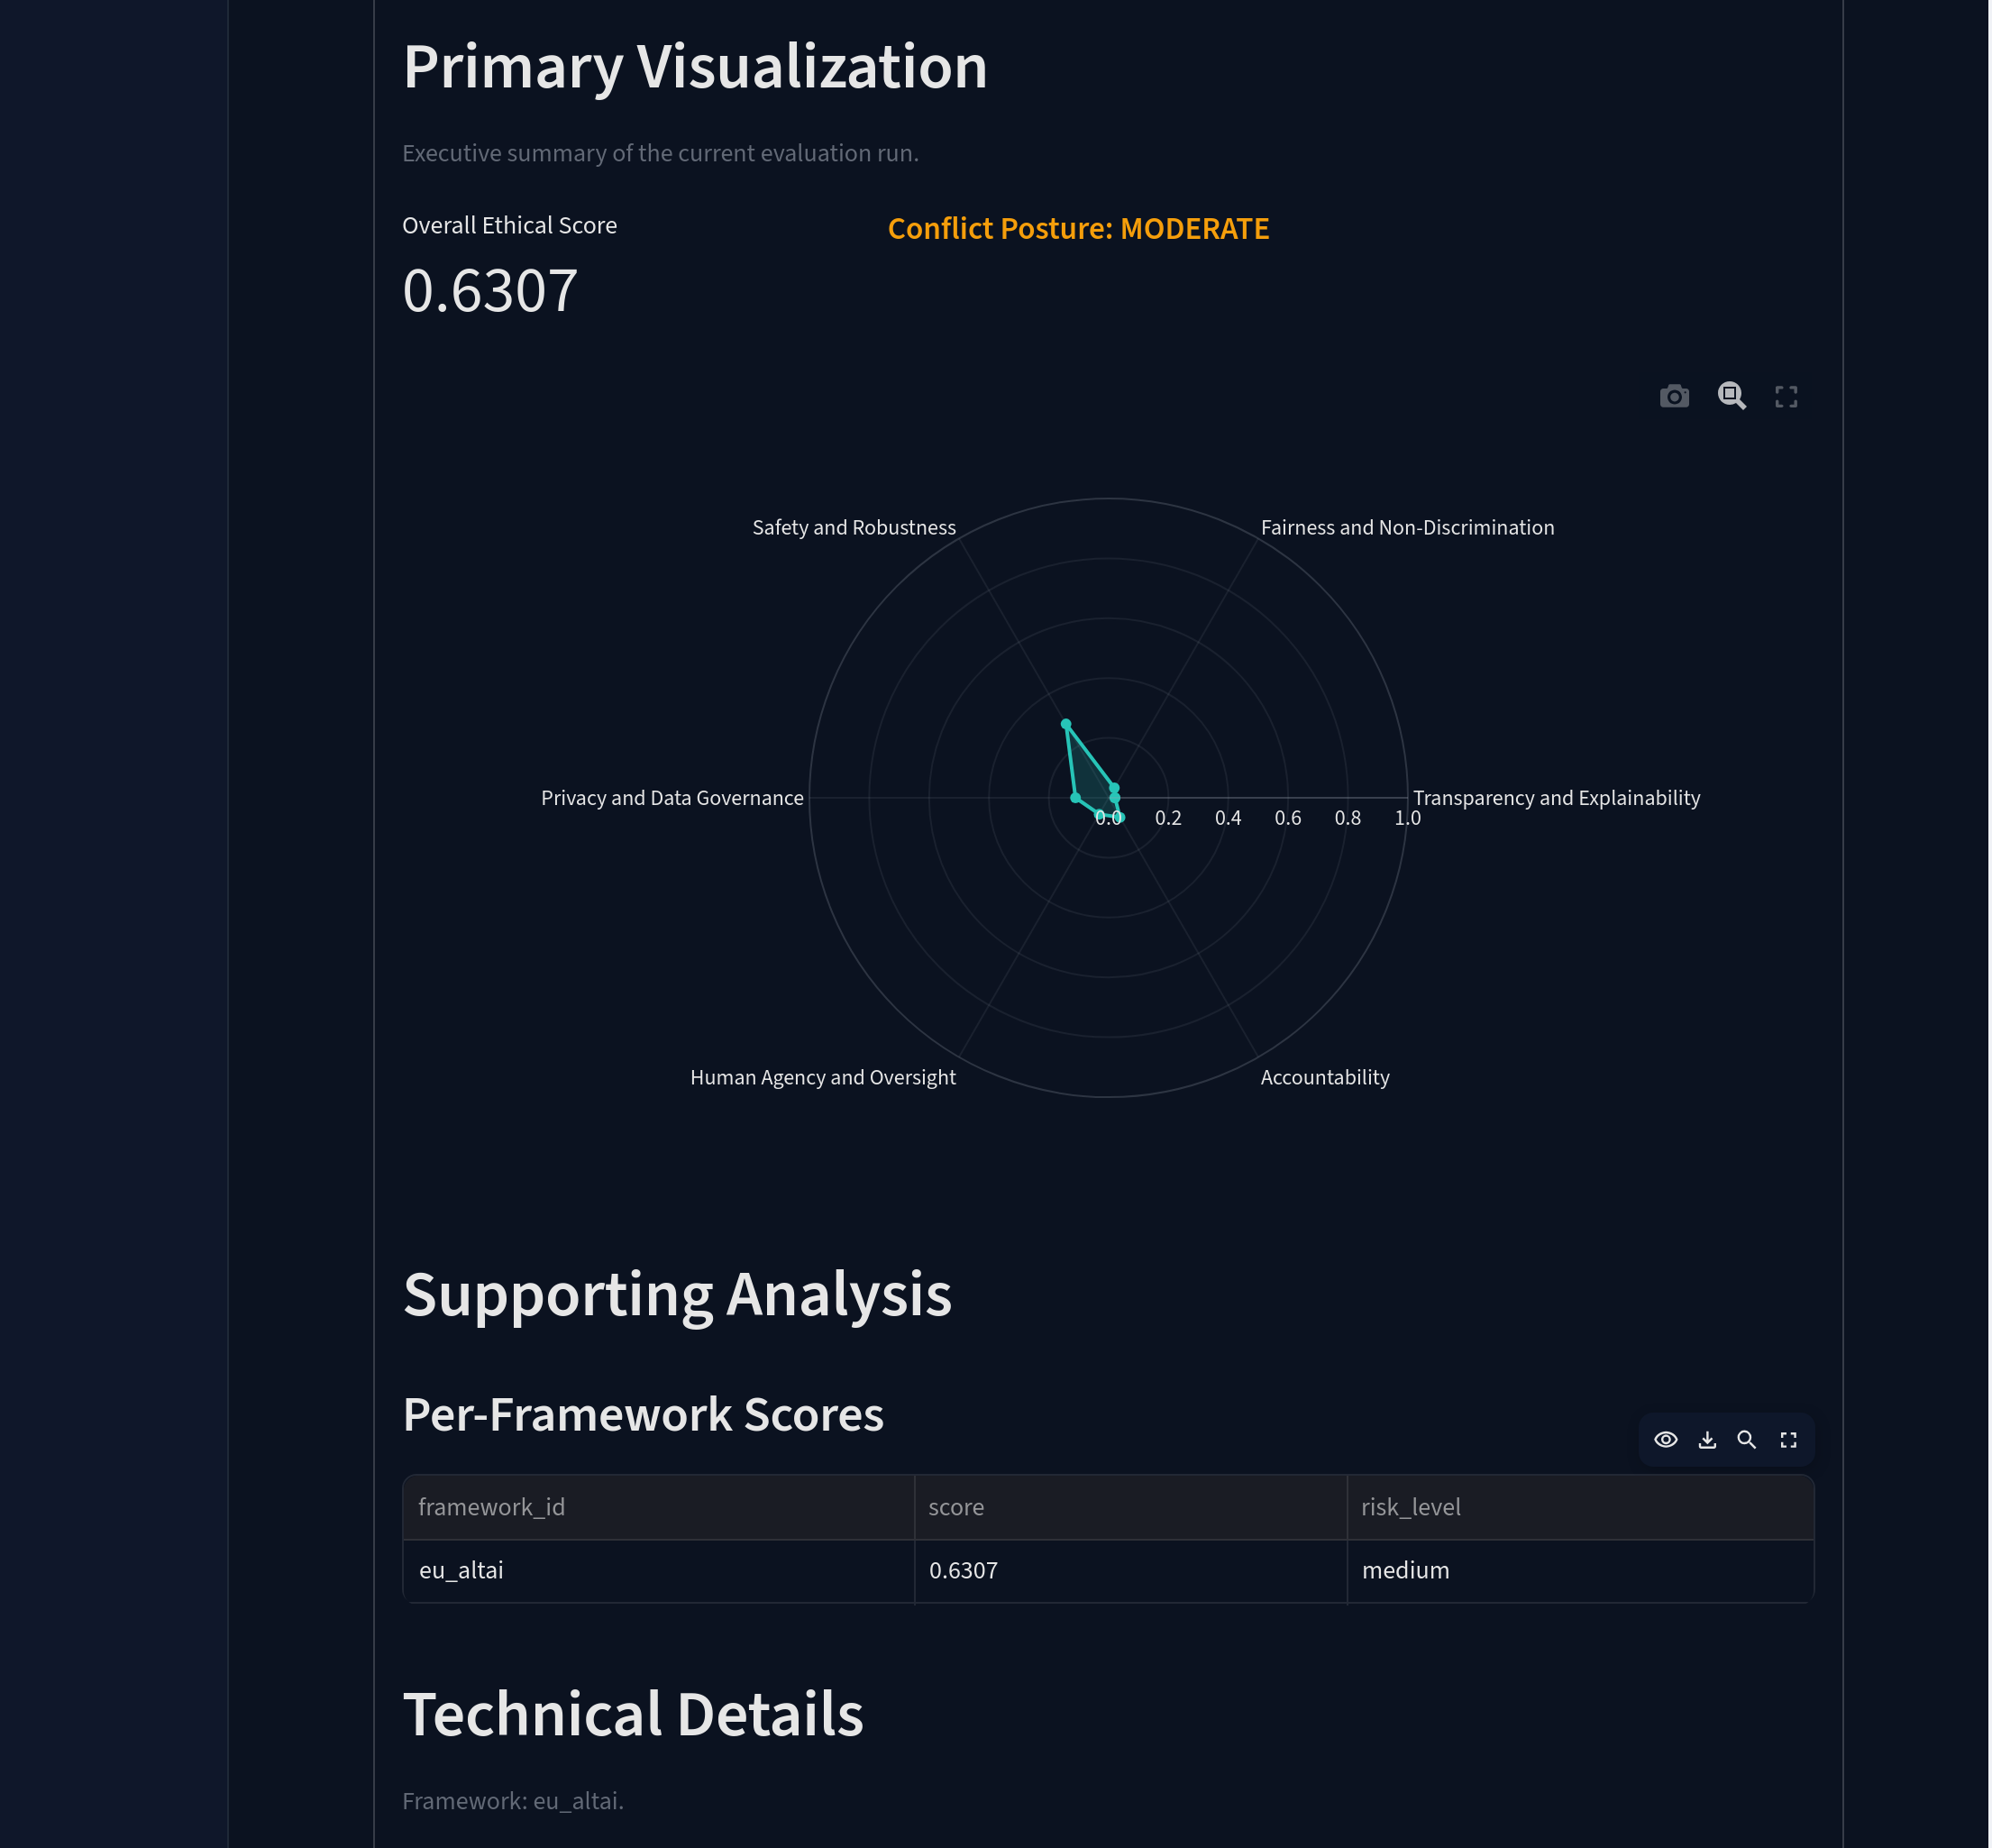
\includegraphics[width=\linewidth,height=0.55\textheight,keepaspectratio]{images/fig_10_2_results.png}

            {\footnotesize Figure 10.2: MEDF evaluation results visualization.}
        \end{column}
    \end{columns}
\end{frame}
% NOTES: Highlight the radar chart shape and the score gauge. Explain that the same
% system scores differently under different frameworks. Approximately 30 seconds.
% Transition: "The platform also detects conflicts between stakeholders."

% ============================================================
% S4: DEMO - CONFLICT AND PARETO
% ============================================================
\begin{frame}{Demo: Conflict Detection and Pareto Resolution}
    \begin{columns}[T]
        \begin{column}{0.48\textwidth}
            \centering
            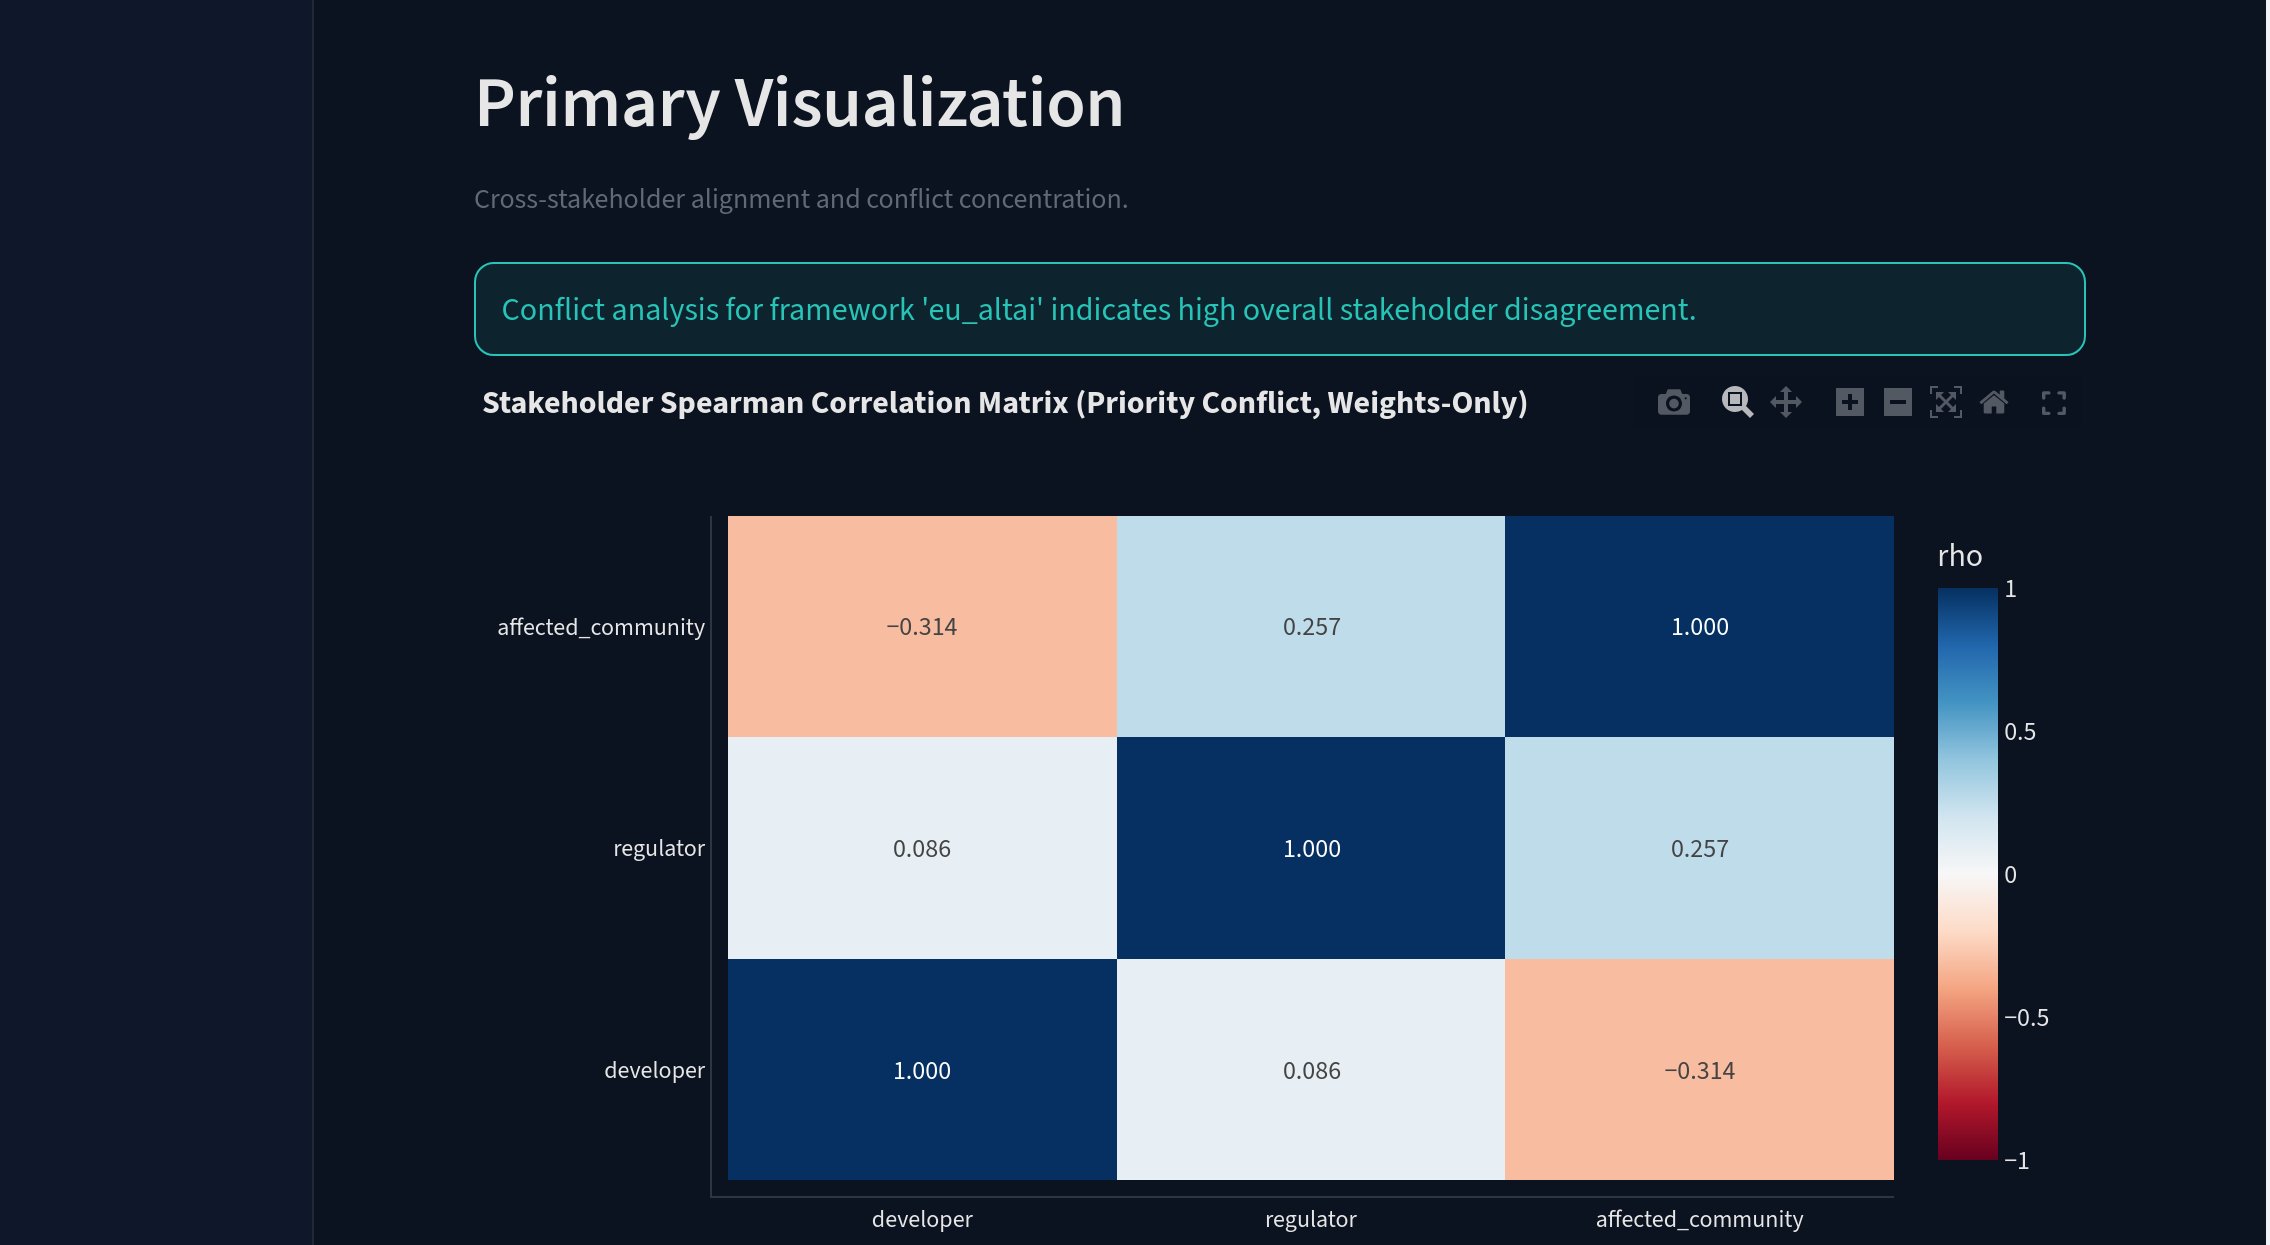
\includegraphics[width=\linewidth,height=0.55\textheight,keepaspectratio]{images/fig_10_3_conflict.png}

            {\footnotesize Figure 10.3: Conflict detection heatmap (Spearman $\rho$).}
        \end{column}
        \begin{column}{0.48\textwidth}
            \centering
            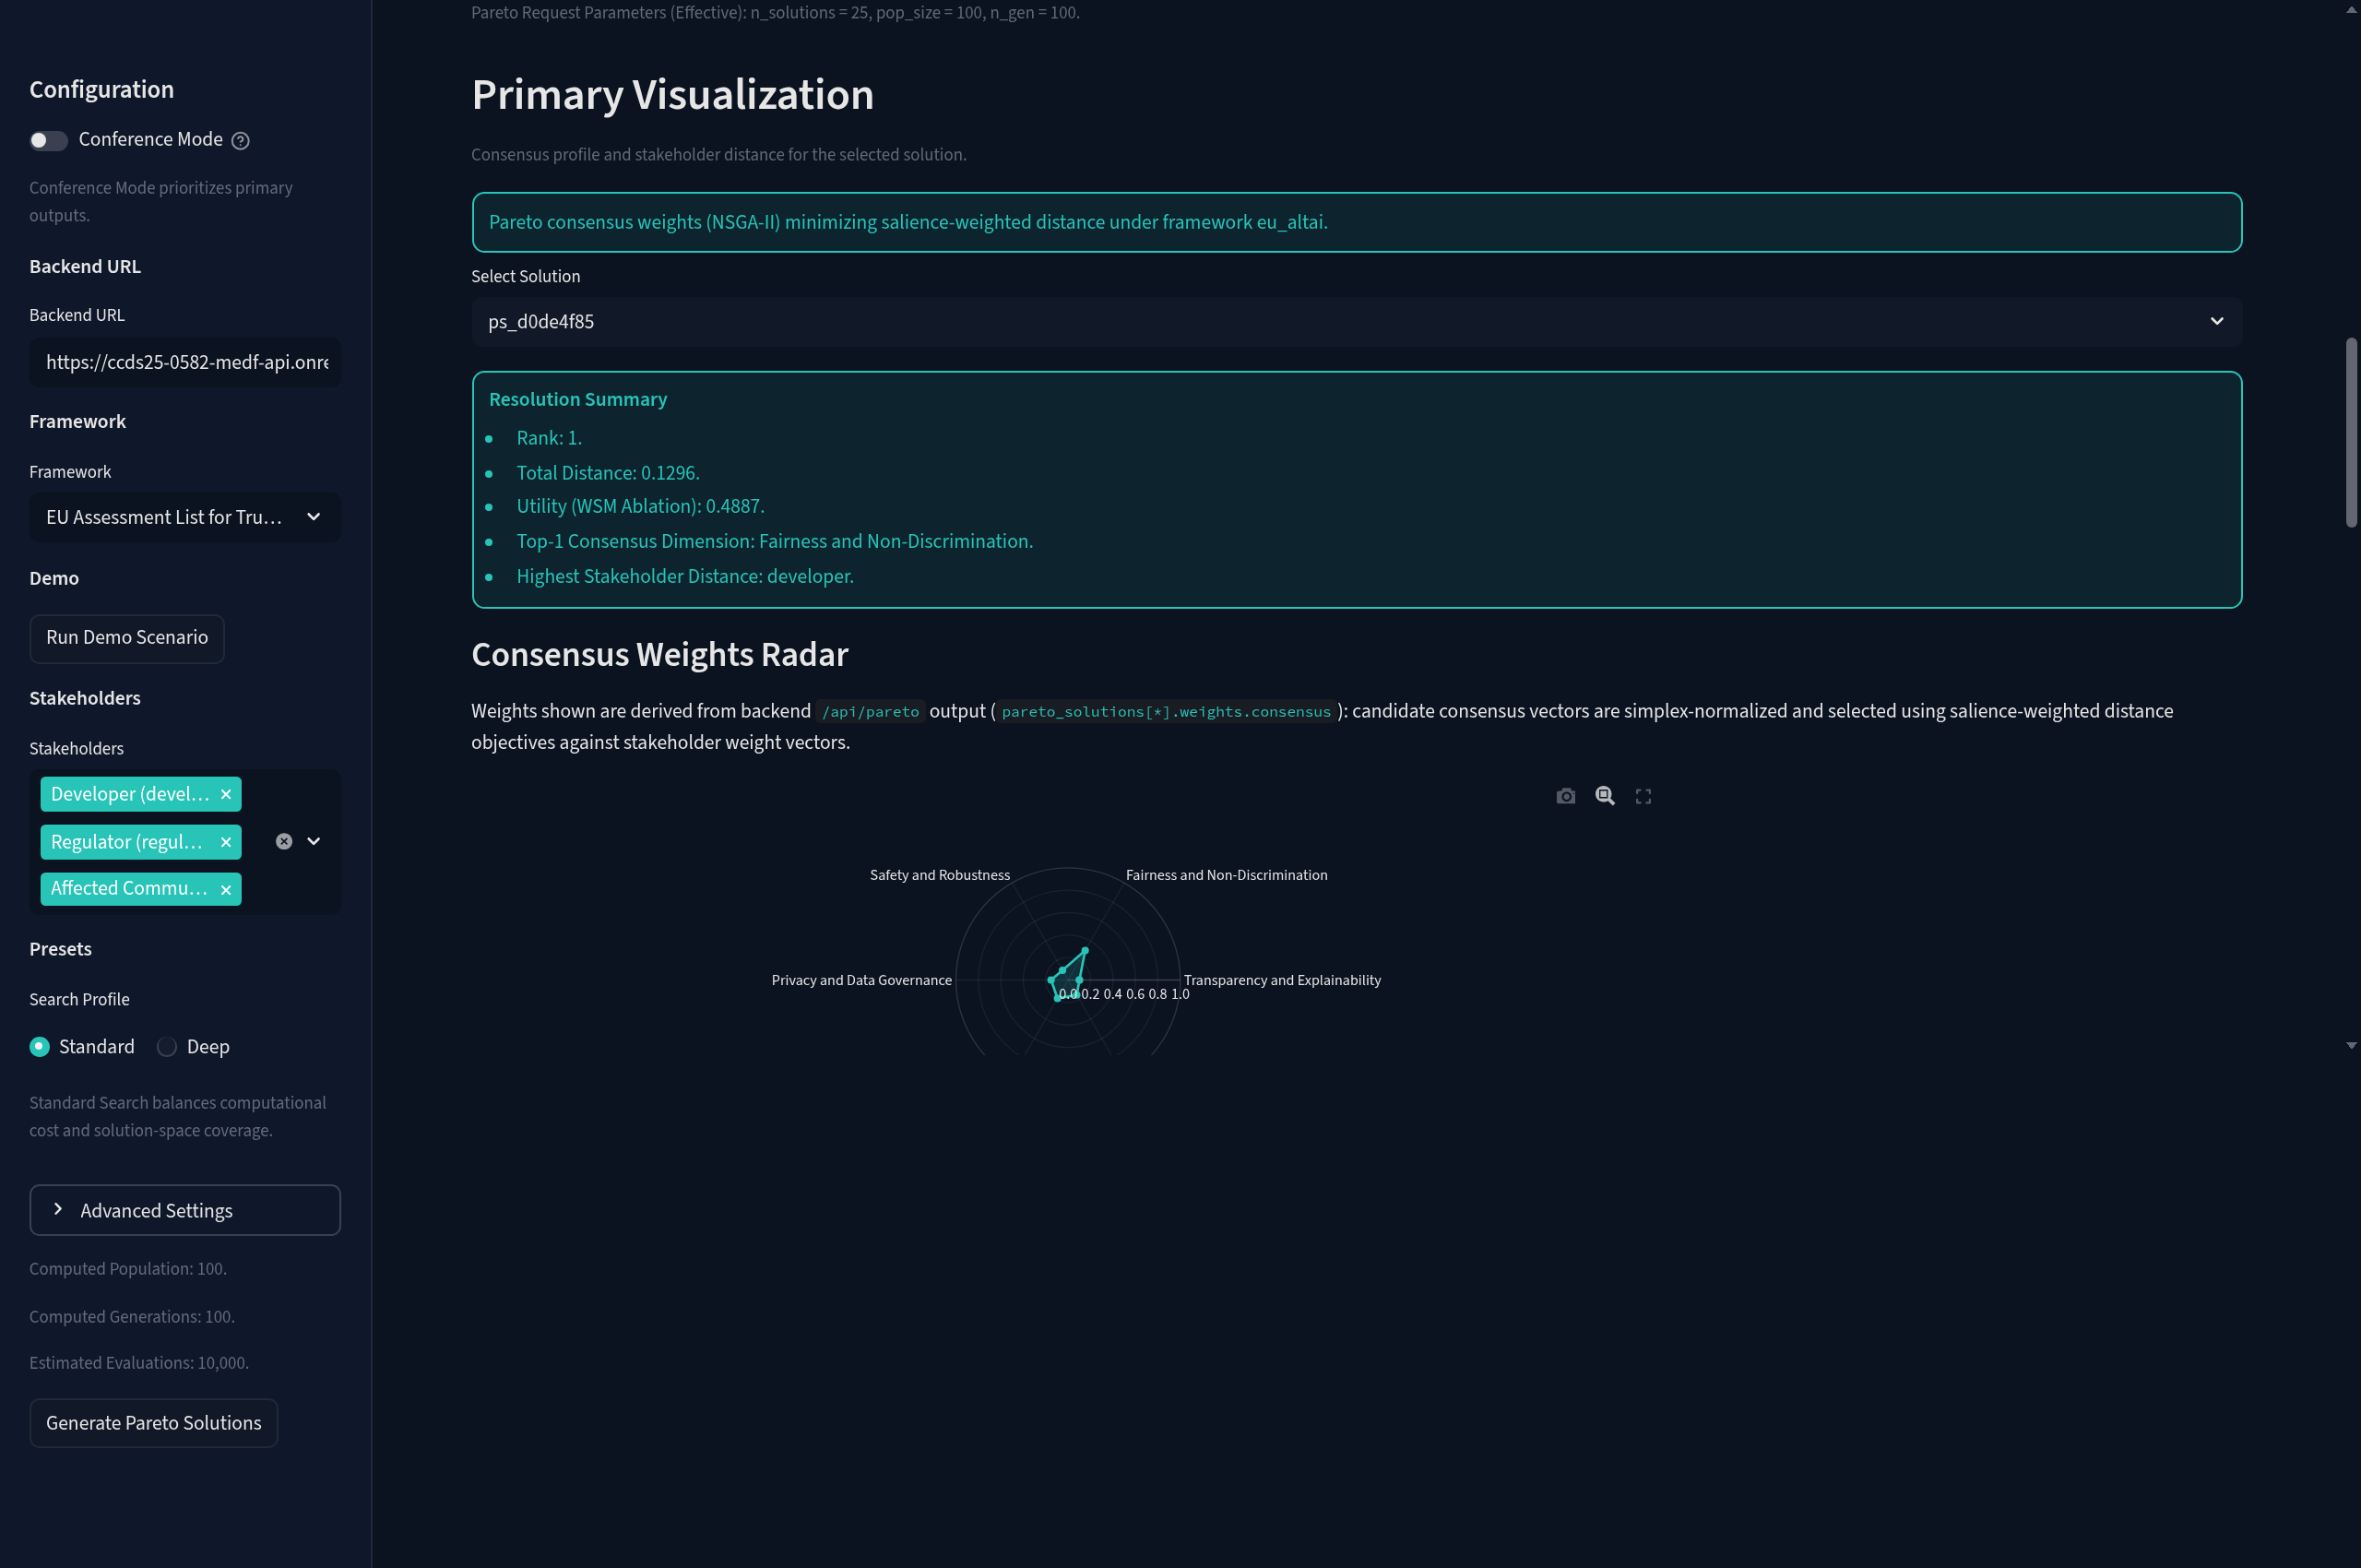
\includegraphics[width=\linewidth,height=0.55\textheight,keepaspectratio]{images/fig_10_4_pareto.png}

            {\footnotesize Figure 10.4: Pareto resolution consensus solutions.}
        \end{column}
    \end{columns}
\end{frame}
% NOTES: Left panel shows where stakeholders agree and disagree. Right panel shows
% NSGA-II generated compromise weight vectors. Approximately 30 seconds.
% Transition: "Now let me provide the context for why this platform was built."

% ============================================================
% S5: OUTLINE
% ============================================================
\begin{frame}{Outline}
    \begin{enumerate}
        \item Platform Demo \textcolor{gray}{(completed)}.
        \item Problem Definition and Gap Analysis.
        \item Methodology, Architecture, and Algorithms.
        \item Case Study Evaluation.
        \item Limitations, Future Work, and Contributions.
    \end{enumerate}
\end{frame}
% NOTES: Brief orientation slide. Approximately 15 seconds.
% Transition: "Let me start with the problem this project addresses."

% ============================================================
% S6: PROBLEM AND MOTIVATION
% ============================================================
\begin{frame}{Problem and Motivation}
    \textbf{Three Interconnected Sub-Problems in AI governance:}
    \begin{enumerate}
        \item \textbf{No standardized metrics.} Ethical concepts remain abstract and context-dependent, making evaluations subjective and incomparable~\cite{mittelstadt2019principles}.
        \item \textbf{Unmanaged stakeholder conflict.} Developers, regulators, and affected communities hold divergent priorities~\cite{freeman1984strategic, mitchell1997stakeholder}.
        \item \textbf{No auditable workflows.} Ethical assessments lack traceability and reproducibility~\cite{hagendorff2020ethics}.
    \end{enumerate}

    \vspace{6pt}
    \textit{Real-World Failures:} facial recognition bias~\cite{buolamwini2018gender}, iTutorGroup age discrimination~\cite{eeoc2022itutorgroup}, NHS-DeepMind privacy breach~\cite{ico2017deepmind}. These patterns are systemic~\cite{oneil2016weapons, raji2020closing}.
\end{frame}
% NOTES: Emphasize these are not hypothetical problems. Each example led to regulatory
% action or public controversy. Approximately 75 seconds.
% Anticipated question: "Why these three sub-problems specifically?"
% Response: "These map directly to the three gaps identified in the literature: Mittelstadt
% showed principles alone fail, Freeman's stakeholder theory shows conflict is structural,
% and Hagendorff found guidelines lack enforcement mechanisms."
% Transition: "No existing tool addresses all three simultaneously."

% ============================================================
% S7: GAP ANALYSIS
% ============================================================
\begin{frame}{Gap Analysis: What Existing Tools Miss}
    \centering
    \footnotesize
    \setlength{\tabcolsep}{3pt}
    \begin{tabular}{l c c c c c c}
        \toprule
        \textbf{Capability} & \textbf{ALTAI} & \textbf{AI Verify} & \textbf{Credo AI} & \textbf{AIF360} & \textbf{Z-Insp.} & \textbf{MEDF} \\
        \midrule
        Cross-framework comparison   & --     & --     & --     & --     & --     & \checkmark \\
        Stakeholder weighting        & --     & --     & --     & --     & --     & \checkmark \\
        Conflict detection           & --     & --     & --     & --     & --     & \checkmark \\
        Pareto consensus             & --     & --     & --     & --     & --     & \checkmark \\
        Quantitative scoring         & --     & \checkmark & \checkmark & \checkmark & --     & \checkmark \\
        Multi-dimensional viz.       & --     & \checkmark & \checkmark & \checkmark & --     & \checkmark \\
        \bottomrule
    \end{tabular}

    \vspace{4pt}
    {\footnotesize Source: Comparative analysis from Chapter~12.3, based on Morley et al.~\cite{morley2020from} and Zicari et al.~\cite{zicari2021zinspection}.}
\end{frame}
% NOTES: This is the novelty defense slide. Stress that MEDF is the only tool offering
% all six capabilities simultaneously. Approximately 60 seconds.
% Anticipated question: "How does MEDF differ from Credo AI?"
% Response: "Credo AI applies separate Policy Packs independently. MEDF compares
% frameworks side-by-side and detects conflicts between stakeholder perspectives,
% which Credo AI does not support."
% Transition: "Let me now describe the methodology behind the platform."


\section{Methodology, Architecture, and Algorithms}

% ============================================================
% S8: METHODOLOGY - DSRM
% ============================================================
\begin{frame}{Methodology: Design Science Research}
    MEDF follows the Design Science Research Methodology (DSRM) by Peffers et al.~\cite{peffers2007dsrm}, providing academic legitimacy beyond pure software engineering.

    \vspace{8pt}
    \begin{enumerate}
        \item \textbf{Problem Identification:} Principles-to-practice gap in AI ethics (Chapters 2--3).
        \item \textbf{Objective Definition:} Quantifiable, multi-stakeholder evaluation (Chapter 3).
        \item \textbf{Design and Development:} Architecture, algorithms, and implementation (Chapters 6--9).
        \item \textbf{Demonstration and Evaluation:} Three real-world case studies (Chapters 10--11).
    \end{enumerate}
\end{frame}
% NOTES: DSRM positions the project as a research artifact, not just code. The six
% DSRM activities map directly onto report chapters. Approximately 60 seconds.
% Transition: "The first design decision was harmonizing three governance frameworks."

% ============================================================
% S9: FRAMEWORK HARMONIZATION
% ============================================================
\begin{frame}{Framework Harmonization: Six Unified Dimensions}
    Three governance frameworks harmonized into one evaluation model.

    \vspace{4pt}
    \begin{columns}[T]
        \begin{column}{0.35\textwidth}
            {\small
            \textbf{Source Frameworks:}
            \begin{itemize}
                \item EU ALTAI~\cite{aihleg2019ethics, aihleg2020altai}.
                \item NIST AI RMF~\cite{nist2023rmf}.
                \item Singapore MGAF~\cite{pdpc2020mgaf}.
            \end{itemize}
            }
        \end{column}
        \begin{column}{0.60\textwidth}
            {\small
            \textbf{Six Unified Dimensions:}
            \begin{enumerate}
                \item Transparency and Explainability.
                \item Fairness and Non-discrimination.
                \item Safety and Robustness.
                \item Privacy and Data Governance.
                \item Human Agency and Oversight.
                \item Accountability.
            \end{enumerate}
            }
        \end{column}
    \end{columns}

    \vspace{6pt}
    {\small Derived from overlapping themes across all three frameworks, informed by Jobin et al.~\cite{jobin2019global}, Floridi et al.~\cite{floridi2018ai4people}, and Zhang et al.~\cite{zhang2023fairness}. Stored as version-controlled YAML files.}
\end{frame}
% NOTES: Explain that the harmonization is a central contribution. Each framework
% assigns different intrinsic weights to each dimension. Approximately 60 seconds.
% Transition: "The system architecture implements this model as a three-tier platform."

% ============================================================
% S10: SYSTEM ARCHITECTURE
% ============================================================
\begin{frame}{System Architecture: Three-Tier Design}
    \begin{columns}[T]
        \begin{column}{0.40\textwidth}
            \begin{itemize}
                \item \textbf{Presentation:} Streamlit dashboard with interactive sliders and radar charts.
                \item \textbf{API/Orchestration Layer:} FastAPI with Pydantic validation, routing, and workflow coordination.
                \item \textbf{Data Layer:} SQLite, YAML registry, and JSON case studies.
            \end{itemize}
        \end{column}
        \begin{column}{0.56\textwidth}
            \centering
            \begin{tikzpicture}[scale=0.78, transform shape,
                node distance=0.55cm,
                layer/.style={rectangle, draw=ntu-blue, fill=ntu-blue!10, text width=5.8cm, minimum height=0.65cm, align=center, font=\small},
                sublayer/.style={rectangle, draw=ntu-blue!50, fill=white, text width=2.6cm, minimum height=0.5cm, align=center, font=\scriptsize},
                arrow/.style={-{Stealth[length=2mm]}, thick, ntu-blue}
            ]
                \node[layer] (pres) {Streamlit Dashboard};
                \node[layer, below=0.4cm of pres] (api) {FastAPI (REST API)};

                \node[sublayer, below left=0.5cm and -0.3cm of api] (eval) {/api/evaluate};
                \node[sublayer, right=0.15cm of eval] (conf) {/api/conflicts};
                \node[sublayer, below right=0.5cm and -0.3cm of api] (par) {/api/pareto};

                \node[layer, below=1.6cm of api] (engine) {Scoring Engine + Harm Assessment};

                \node[layer, below=0.4cm of engine] (data) {YAML Registry | SQLite | Case Study JSON};

                \draw[arrow] (pres) -- node[right, font=\scriptsize]{REST} (api);
                \draw[arrow] (api) -- (eval);
                \draw[arrow] (api) -- (conf);
                \draw[arrow] (api) -- (par);
                \draw[arrow] (engine) -- (data);
                \draw[arrow, dashed] (eval.south) -- ++(0,-0.25) -| (engine.north west);
                \draw[arrow, dashed] (par.south) -- ++(0,-0.25) -| (engine.north east);
            \end{tikzpicture}
        \end{column}
    \end{columns}
\end{frame}
% NOTES: Emphasize clean separation of concerns. The Streamlit frontend communicates
% exclusively through the REST API. The routers (evaluate.py, conflicts.py, pareto.py)
% belong to the API/orchestration layer, handling routing, request validation, and
% workflow coordination. The scoring engine and harm assessment module form the engine
% layer, containing the analysis, scoring, and optimization logic. Note the acknowledged
% technical debt: conflict analysis logic currently resides in the API router layer,
% not in a standalone engine module. Approximately 60 seconds.
% Transition: "The scoring engine at the core uses TOPSIS with a product pooling mechanism."

% ============================================================
% S11: ALGORITHM - TOPSIS SCORING ENGINE
% ============================================================
\begin{frame}{Algorithm: TOPSIS Scoring Engine}
    \textbf{Product Pooling} combines stakeholder and framework weights~\cite{hwang1981multiple, behzadian2012topsis}:
    \[
        w_{\text{eff}} \propto w_s \odot w_f
    \]

    \textbf{TOPSIS Closeness Coefficient} (distance to ideal vs.\ anti-ideal):
    \[
        C = \frac{d^-}{d^+ + d^-} \quad \in [0, 1]
    \]

    \vspace{6pt}
    \begin{itemize}
        \item Single-alternative evaluation uses synthetic best/worst anchors to keep $C$ well-defined.
        \item Risk classification: $C \geq 0.80$ Low, $0.60$--$0.80$ Medium, $0.40$--$0.60$ High, $< 0.40$ Critical.
    \end{itemize}
\end{frame}
% NOTES: Product pooling ensures a dimension scores high only if BOTH the stakeholder
% and the framework consider it important. The synthetic anchor trick is a critical
% adaptation for single-system evaluation. Approximately 90 seconds.
% Anticipated question: "Why TOPSIS over AHP or VIKOR?"
% Response: "TOPSIS is computationally efficient, produces a clear scalar score, and
% performs favorably against VIKOR in comparative analyses. AHP requires pairwise
% comparisons that would burden the user interface."
% Transition: "The conflict detection module uses Spearman rank correlation."

% ============================================================
% S12: ALGORITHM - CONFLICT DETECTION
% ============================================================
\begin{frame}{Algorithm: Conflict Detection (Spearman $\rho$)}
    MEDF computes two types of stakeholder correlation.

    \vspace{6pt}
    \begin{enumerate}
        \item \textbf{Priority Conflict (Weights-Only):} Spearman $\rho$ between raw stakeholder weight vectors. Measures general agreement on dimension importance.
        \item \textbf{System-Salience Conflict (Contribution-Based):} Spearman $\rho$ between contribution vectors (effective weights $\times$ dimension scores). Measures agreement for a specific AI system.
    \end{enumerate}

    \vspace{6pt}
    \textbf{Critical Insight:} The contribution-based metric produces different conflict levels across case studies, even with identical stakeholder weights. This captures case-specific dynamics.
\end{frame}
% NOTES: The distinction between these two metrics is a differentiating feature.
% Contribution-based conflict is what makes the analysis system-aware.
% Approximately 60 seconds.
% Transition: "When conflict is high, MEDF generates Pareto-optimal consensus solutions."

% ============================================================
% S13: ALGORITHM - PARETO AND HARM
% ============================================================
\begin{frame}{Algorithm: Pareto Consensus and Harm Assessment}
    \textbf{NSGA-II} objective function with salience weighting~\cite{deb2002nsga}:
    \[
        f_k(w_c) = \sum_i s_i \cdot |w_{c,i} - w_{k,i}|
    \]

    \textbf{Harm Score} combines system performance and governance disagreement:
    \[
        h = 0.7 \times (1 - s_{\text{norm}}) + 0.3 \times \bar{d}
    \]

    \vspace{4pt}
    \begin{itemize}
        \item The 0.7/0.3 split reflects a design decision: system performance dominates risk classification, with stakeholder disagreement as an aggravating factor.
    \end{itemize}
\end{frame}
% NOTES: The salience factor s_i ensures the optimizer prioritizes dimensions that
% matter most for the system under evaluation. The harm score is a composite metric.
% Approximately 45 seconds.
% Transition: "Let me now present the three case studies used to validate the platform."


\section{Case Study Evaluation}

% ============================================================
% S14: CASE STUDY 1 - FACIAL RECOGNITION
% ============================================================
\begin{frame}{Case Study 1: Metropolitan Police Live Facial Recognition}
    \begin{columns}[T]
        \begin{column}{0.48\textwidth}
            \textbf{Baseline Scores:} Fairness 1.5, Privacy 1.5, Safety 5.0 (1--7 Likert scale).

            \vspace{6pt}
            \textbf{Results (All Frameworks):}
            \begin{itemize}
                \item Overall: \textbf{0.3866} (Critical).
                \item Developer: 0.4826.
                \item Affected Community: 0.3063.
            \end{itemize}

            \vspace{6pt}
            \textbf{Conflict:} Low (all $\rho > 0.89$). The extreme ethical profile creates clear ranking agreement.
        \end{column}
        \begin{column}{0.48\textwidth}
            \centering
            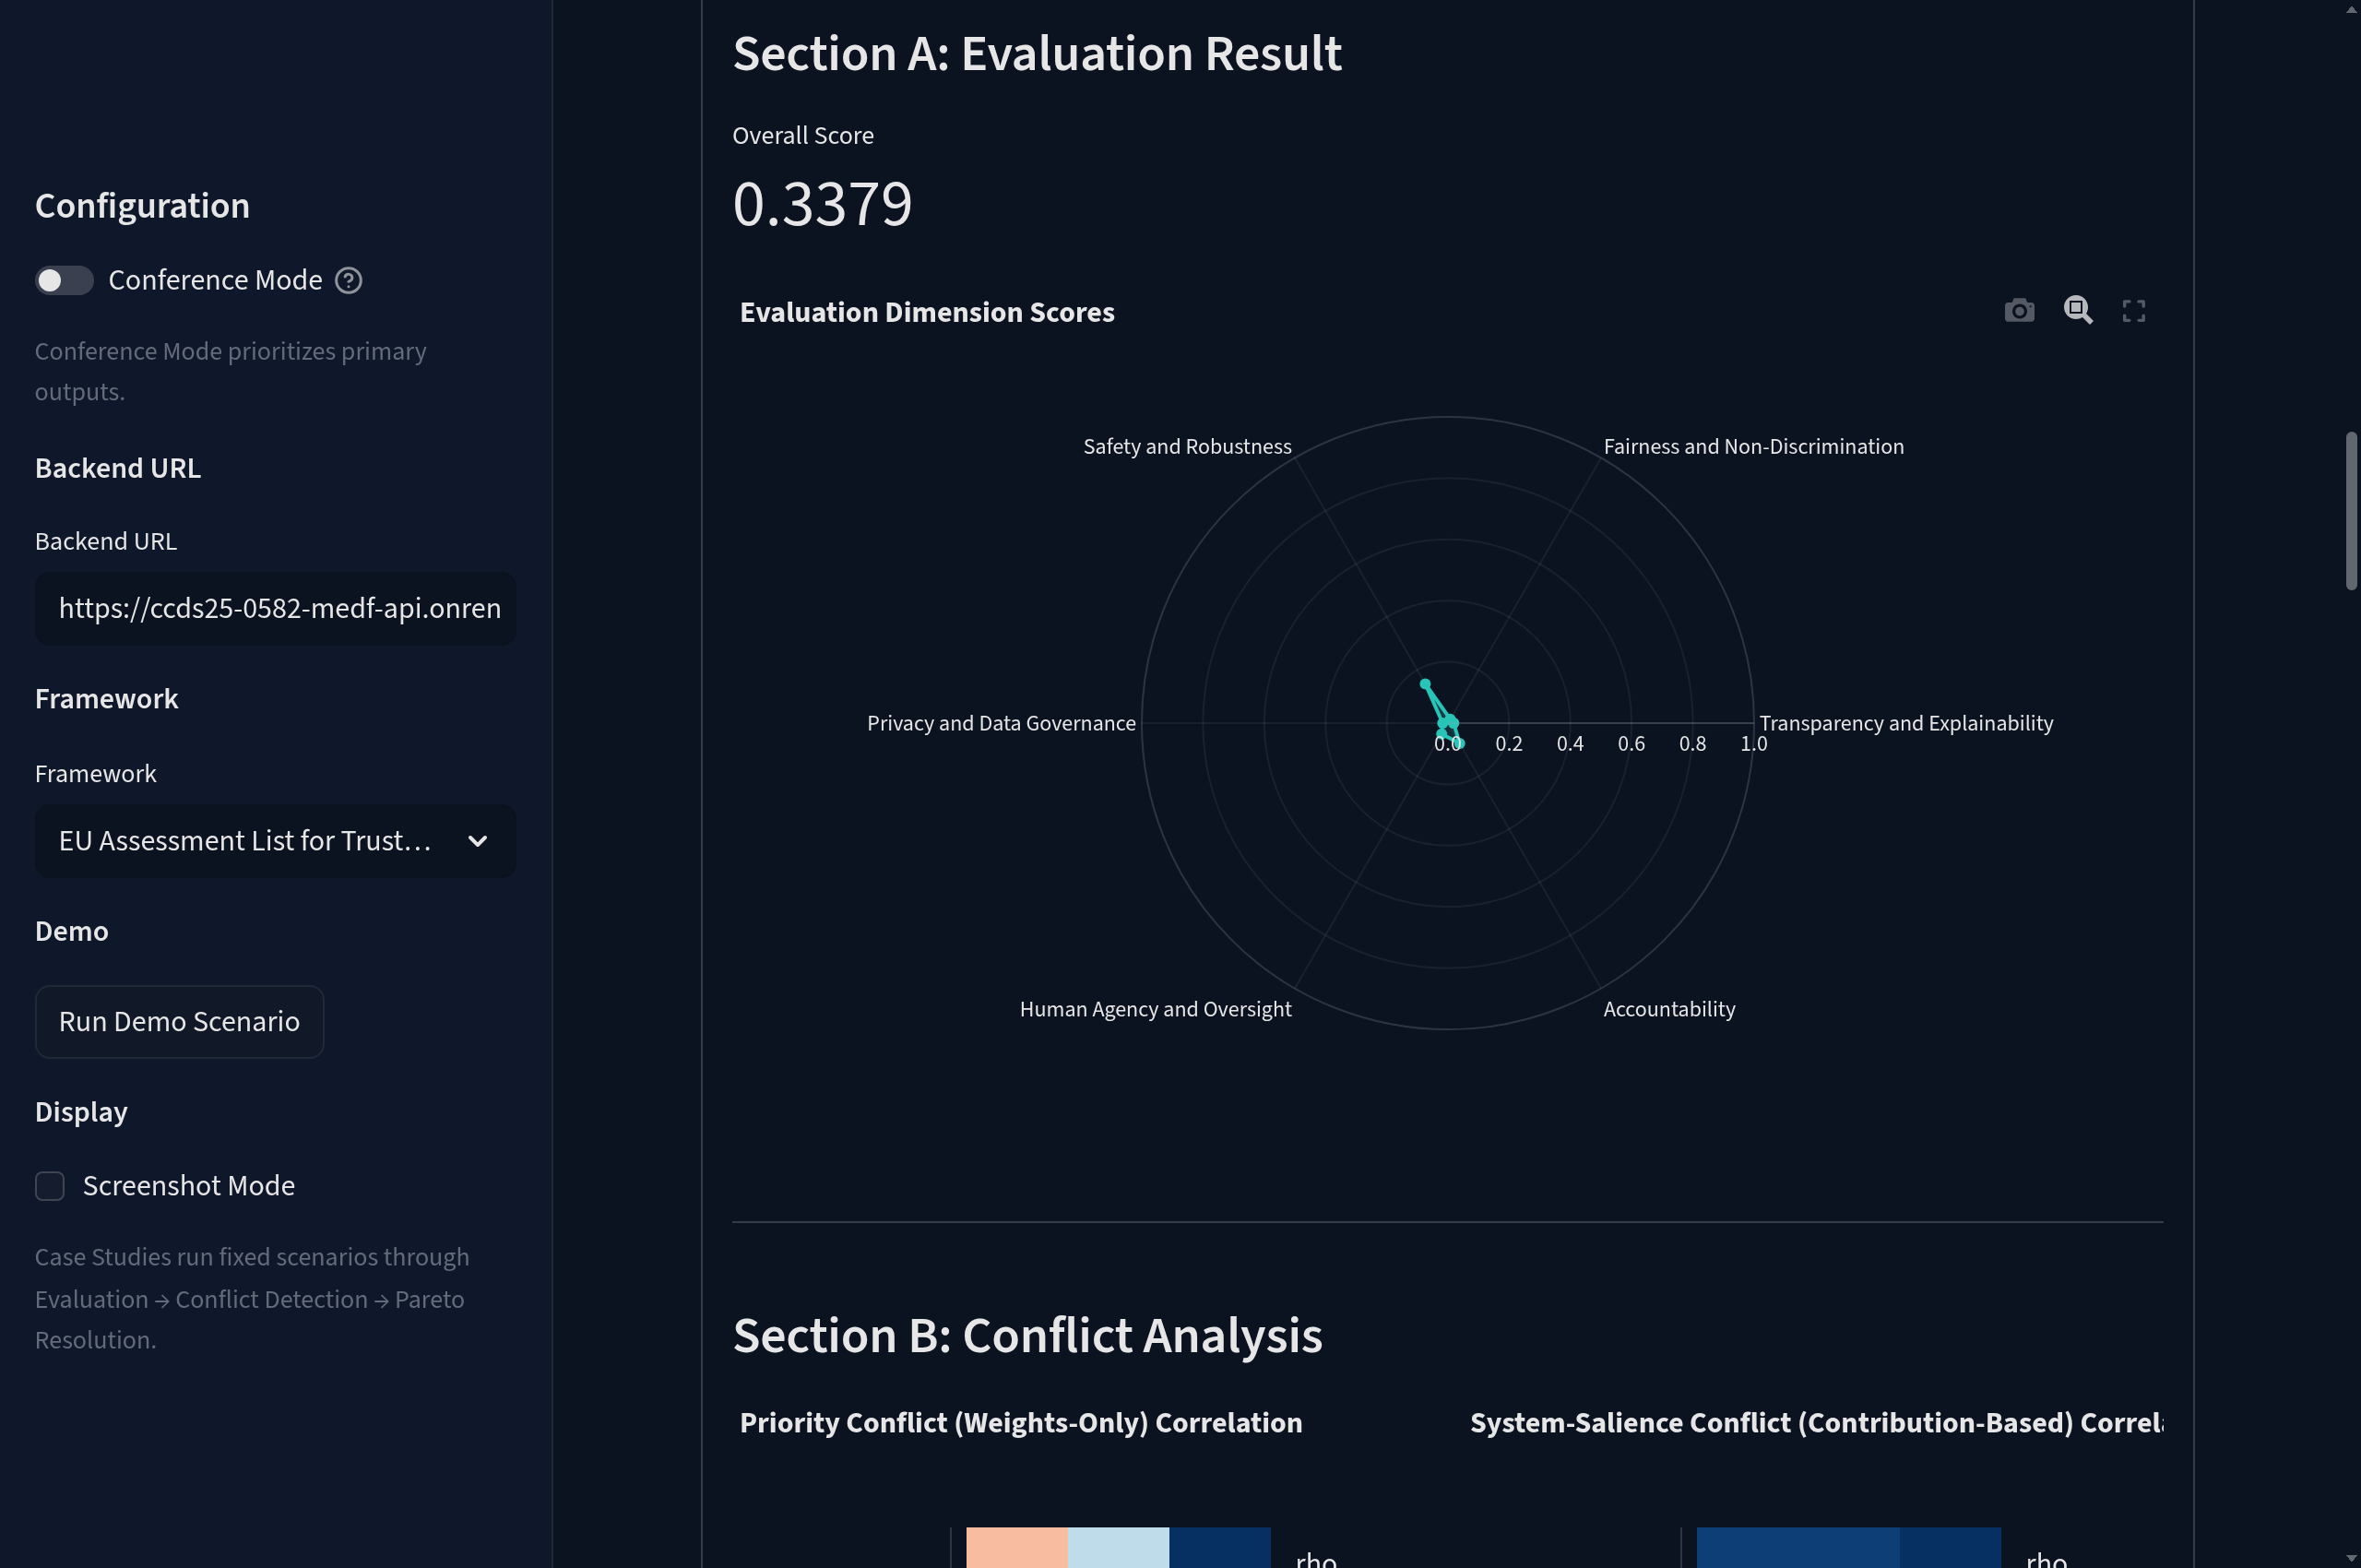
\includegraphics[width=\linewidth,height=0.55\textheight,keepaspectratio]{images/fig_10_6_casestudy1.png}

            {\footnotesize Figure 10.6: Case Study 1 evaluation results (overall score 0.3379).}
        \end{column}
    \end{columns}
\end{frame}
% NOTES: The facial recognition case has severe failures on Fairness and Privacy.
% Despite different absolute scores, all stakeholders agree on the dimension ranking.
% Approximately 60 seconds.
% Transition: "The hiring algorithm case shows a different conflict pattern."

% ============================================================
% S15: CASE STUDY 2 - HIRING ALGORITHM
% ============================================================
\begin{frame}{Case Study 2: iTutorGroup Automated Hiring}
    \textbf{System Description:} Automated rejection of applicants over age 55~\cite{eeoc2022itutorgroup}. Deliberate, systemic age discrimination.

    \vspace{8pt}
    \textbf{MEDF Evaluation Results (All Frameworks):}
    \begin{itemize}
        \item Overall: \textbf{0.3477} (Critical risk). A single catastrophic ethical flaw renders the system unacceptable from every stakeholder perspective.
        \item Conflict: Moderate ($\rho = 0.54$ Developer-Regulator). The ambiguous ethical profile exposes genuine disagreement.
        \item The Regulator scores higher (0.4004) due to Accountability emphasis, while the Affected Community scores lowest (0.3005).
    \end{itemize}
\end{frame}
% NOTES: This case demonstrates MEDF's ability to correctly penalize systems with
% catastrophic single-dimension failures. Approximately 60 seconds.
% Transition: "The NHS-DeepMind case reveals the highest stakeholder conflict."

% ============================================================
% S16: CASE STUDY 3 - NHS-DEEPMIND
% ============================================================
\begin{frame}{Case Study 3: Royal Free NHS-DeepMind Streams}
    \textbf{System Description:} Clinical AKI detection app. Life-saving benefit, but 1.6M patient records accessed without consent~\cite{ico2017deepmind}.

    \vspace{8pt}
    \textbf{MEDF Evaluation Results (All Frameworks):}
    \begin{itemize}
        \item Overall: \textbf{0.6003} (Medium risk). The genuine clinical benefit (Safety 6.0) partially offsets the Privacy failure (3.5).
        \item Conflict: High ($\rho = -0.14$ Developer-Regulator). The balanced ethical profile exposes real stakeholder tension.
        \item This is the most genuinely contentious case: the Developer values clinical utility while the Regulator prioritizes data governance.
    \end{itemize}
\end{frame}
% NOTES: This case demonstrates the full power of the contribution-based conflict metric.
% Unlike the facial recognition case, the balanced profile here exposes genuine disagreement.
% Approximately 60 seconds.
% Transition: "Comparing all three cases reveals the critical finding of this project."

% ============================================================
% S17: CROSS-CASE COMPARISON
% ============================================================
\begin{frame}{Cross-Case Comparative Analysis}
    \centering
    \setlength{\tabcolsep}{4pt}
    \begin{tabular}{l c c c c}
        \toprule
        \textbf{Case Study} & \textbf{Overall} & \textbf{Risk} & \textbf{Min $\rho$} & \textbf{Conflict} \\
        \midrule
        Facial Recognition   & 0.3866 & Critical & 0.89  & Low \\
        iTutorGroup Hiring   & 0.3477 & Critical & 0.54  & Moderate \\
        NHS-DeepMind Streams & 0.6003 & Medium   & $-0.14$ & High \\
        \bottomrule
    \end{tabular}

    \vspace{8pt}
    {\small \textbf{Critical Finding:} Contribution-based conflict analysis differentiates genuinely contentious cases from clear ethical violations, even when using identical default stakeholder weights.}
\end{frame}
% NOTES: This table is the summary artifact for the case study evaluation. The inverse
% relationship between ethical severity and conflict level is the central insight.
% Approximately 60 seconds.
% Transition: "Let me now address the limitations of this work."


\section{Limitations, Future Work, and Contributions}

% ============================================================
% S18: LIMITATIONS
% ============================================================
\begin{frame}{Limitations}
    \begin{enumerate}
        \item \textbf{Input Subjectivity.} Baseline dimension scores and stakeholder weights are user-provided. No built-in mechanism verifies their accuracy against ground truth.
        \item \textbf{Linearity and Independence Assumptions.} TOPSIS and WSM assume dimensions are independent. In reality, improving transparency can affect accountability.
        \item \textbf{No Primary User Research.} The project scope excluded user surveys, interviews, and statistical user studies.
        \item \textbf{Router-Level Technical Debt.} Conflict analysis logic remains in the API router layer rather than an extracted standalone engine module.
    \end{enumerate}
\end{frame}
% NOTES: State limitations early and honestly (per Dr. Zhang's alignment rules).
% These do not invalidate the approach but define its boundaries.
% Approximately 45 seconds.
% Transition: "These limitations define clear directions for future work."

% ============================================================
% S19: FUTURE WORK
% ============================================================
\begin{frame}{Future Work}
    \begin{enumerate}
        \item \textbf{NLP-Based Automated Scoring.} Generate baseline dimension scores from system documentation and audit reports, reducing reliance on subjective manual input.
        \item \textbf{CI/CD Pipeline Integration.} Embed MEDF evaluations as automated ethical checks in the software development workflow.
        \item \textbf{Empirical User Studies.} Validate usability and perceived value with AI practitioners, ethicists, and policymakers.
        \item \textbf{Expanded Framework Library.} Add IEEE Ethically Aligned Design, OECD AI Principles, and sector-specific regulations.
    \end{enumerate}
\end{frame}
% NOTES: Each future work item addresses a specific limitation. NLP scoring addresses
% input subjectivity. CI/CD integration addresses the post-hoc evaluation limitation.
% Approximately 30 seconds.
% Transition: "To summarize, this project makes five concrete contributions."

% ============================================================
% S20: CONTRIBUTIONS (FINAL SLIDE)
% ============================================================
\begin{frame}{Contributions}
    \begin{enumerate}
        \item \textbf{Unified Six-Dimension Model} harmonizing EU ALTAI, NIST AI RMF, and Singapore MGAF into a single coherent evaluation framework.
        \item \textbf{TOPSIS/WSM Scoring Engine} with product pooling for integrated stakeholder-framework weight computation.
        \item \textbf{Contribution-Based Conflict Detection} via Spearman rank correlation, producing case-sensitive stakeholder disagreement analysis.
        \item \textbf{NSGA-II Pareto Consensus Generation} for multi-stakeholder mediation with salience-weighted objective functions.
        \item \textbf{Open-Source, Reproducible Platform} with 50+ automated tests, public deployment, and complete documentation.
    \end{enumerate}
\end{frame}
% NOTES: End on this slide. Do not advance to a "Thank You" slide. Let the
% contributions remain visible as the examiners formulate their questions.
% Approximately 45 seconds. Total presentation time: approximately 18.5 minutes.
% Anticipated question: "What is your single most important contribution?"
% Response: "The contribution-based conflict detection metric. It is the mechanism
% that differentiates genuinely contentious cases from clear violations, which no
% existing tool provides."



\begin{frame}[allowframebreaks]{References}
    \setbeamertemplate{frametitle continuation}[from second]
    \footnotesize
    \printbibliography[heading=none]
\end{frame}


% ============================================================
% BACKUP SLIDES (for Q&A)
% ============================================================
\appendix
\section{Backup Slides}

\begin{frame}{Backup: Module Dependency Diagram}
    \centering
    \begin{tikzpicture}[scale=0.60, transform shape,
        node distance=0.8cm,
        mod/.style={rectangle, draw=ntu-blue, fill=ntu-blue!10, text width=3.5cm, minimum height=0.6cm, align=center, font=\footnotesize\ttfamily},
        arrow/.style={-{Stealth[length=2mm]}, thick, ntu-blue!70}
    ]
        % Row 1: Entry point
        \node[mod] (main) {main.py};

        % Row 2: API/Router layer (evenly spaced)
        \node[mod, below left=0.8cm and 1.5cm of main] (eval) {routers/evaluate.py};
        \node[mod, below=0.8cm of main] (conf) {routers/conflicts.py};
        \node[mod, below right=0.8cm and 1.5cm of main] (par) {routers/pareto.py};

        % Row 3: Engine layer
        \node[mod, below=0.8cm of $(eval)!0.5!(conf)$] (scoring) {scoring\_engine.py};
        \node[mod, below=0.8cm of $(conf)!0.5!(par)$] (harm) {harm\_assessment.py};

        % Row 4: Data layer
        \node[mod, below=0.8cm of scoring] (models) {models.py};
        \node[mod, below=0.8cm of harm] (registry) {framework\_registry.py};

        % All arrows point strictly downward
        \draw[arrow] (main) -- (eval);
        \draw[arrow] (main) -- (conf);
        \draw[arrow] (main) -- (par);
        \draw[arrow] (eval) -- (scoring);
        \draw[arrow] (conf) -- (scoring);
        \draw[arrow] (par) -- (harm);
        \draw[arrow] (scoring) -- (models);
        \draw[arrow] (harm) -- (registry);
    \end{tikzpicture}
\end{frame}
% NOTES: This corresponds to Figure 7.2 in the report. Note the acknowledged
% technical debt: conflict analysis logic currently resides in the API router layer,
% not in a standalone engine module.

\begin{frame}{Backup: End-to-End Evaluation Pipeline}
    \centering
    \begin{tikzpicture}[scale=0.78, transform shape,
        node distance=0.9cm,
        block/.style={rectangle, draw=ntu-blue, fill=ntu-blue!10, text width=4.2cm, minimum height=0.7cm, align=center, font=\small},
        arrow/.style={-{Stealth[length=2.5mm]}, thick, ntu-blue}
    ]
        \node[block] (input1) {AI System Scores};
        \node[block, right=1.5cm of input1] (input2) {Stakeholder Weights};
        \node[block, below=of $(input1)!0.5!(input2)$] (ew) {Compute Effective Weights};
        \node[block, below=of ew] (score) {TOPSIS / WSM Scoring};
        \node[block, below=of score] (agg) {Aggregate Across Frameworks};
        \node[block, below left=0.8cm and 0.3cm of agg] (conflict) {Conflict Detection\\(Spearman $\rho$)};
        \node[block, below right=0.8cm and 0.3cm of agg] (harm) {Harm Assessment};
        \node[block, below=1.2cm of agg] (result) {Evaluation Result};

        \draw[arrow] (input1) -- (ew);
        \draw[arrow] (input2) -- (ew);
        \draw[arrow] (ew) -- (score);
        \draw[arrow] (score) -- (agg);
        \draw[arrow] (agg) -- (conflict);
        \draw[arrow] (agg) -- (harm);
        \draw[arrow] (conflict) -- (result);
        \draw[arrow] (harm) -- (result);
    \end{tikzpicture}
\end{frame}
% NOTES: This corresponds to Figure 8.2 in the report. The pipeline is deterministic
% and sequential, ensuring reproducibility.

\begin{frame}{Backup: Stakeholder Weight Profiles}
    \centering
    \footnotesize
    \setlength{\tabcolsep}{4pt}
    \begin{tabular}{l c c c}
        \toprule
        \textbf{Dimension} & \textbf{Developer} & \textbf{Regulator} & \textbf{Affected Community} \\
        \midrule
        Transparency        & 0.10 & 0.20 & 0.10 \\
        Fairness            & 0.15 & 0.20 & 0.30 \\
        Safety              & 0.30 & 0.10 & 0.10 \\
        Privacy             & 0.15 & 0.15 & 0.15 \\
        Human Oversight     & 0.15 & 0.10 & 0.20 \\
        Accountability      & 0.15 & 0.25 & 0.15 \\
        \midrule
        \textbf{Total}      & 1.00 & 1.00 & 1.00 \\
        \bottomrule
    \end{tabular}
\end{frame}
% NOTES: Reference Table 11.1 in the report. Developers emphasize Safety (0.30).
% Regulators emphasize Accountability (0.25). Affected Communities emphasize Fairness (0.30).

\begin{frame}{Backup: Framework Weight Vectors}
    \centering
    \resizebox{0.85\linewidth}{!}{%
    \footnotesize
    \setlength{\tabcolsep}{4pt}
    \begin{tabular}{l c c c}
        \toprule
        \textbf{Dimension} & \textbf{EU ALTAI} & \textbf{NIST RMF} & \textbf{SG MGAF} \\
        \midrule
        Transparency        & 0.09 & 0.11 & 0.25 \\
        Fairness            & 0.14 & 0.11 & 0.10 \\
        Safety              & 0.23 & 0.26 & 0.15 \\
        Privacy             & 0.23 & 0.11 & 0.10 \\
        Human Oversight     & 0.18 & 0.11 & 0.20 \\
        Accountability      & 0.14 & 0.32 & 0.20 \\
        \midrule
        \textbf{Total}      & 1.01 & 1.02 & 1.00 \\
        \bottomrule
    \end{tabular}%
    }

    \vspace{6pt}
    {\centering\small Weights derived from the structural emphasis of each framework (sub-item counts).\par}
\end{frame}
% NOTES: These intrinsic weights come from Appendix B of the report.
% Each framework emphasizes different dimensions based on its regulatory philosophy.

\end{document}
